\section{Evaluation}
\label{s:evaluation}


%1. Collect terms
%2. Query search results.
%3. Crawl data and get ground truth (how
%many).
%4. Train model and select parameters use 5-fold stratified cross validation
%~\cite{scikit-learn}.

In the above section ~\autoref{s:methodology}, we propose the SWM and explains
how it can be used to do cloaking detection (outlier detection). There are three
parameters to be learned, the upper bound of inconsistent coefficient in
clustering phase $T_{learn}$, the lower bound of inconsistent coefficient in the detection
phase $T_{detect}$, the fix parameter minimum radius $R_{detect}$. 
In order to measure cloaking in both SEO and SEM, we collects four candidate dataset
~\autoref{ss:dataset}. In this section,
we first describe the groundtruth obtained from $D_{hot, search}$ and $D_{spam,
search}$, then use it to train and test the performance of the proposed model.

\subsection{Groundtruth}

%We randomly sample 600 websites from the dataset, for 10 times. This results in
%5726 websites. We manually label them and \XXX{cloaking}, \XXX{not}, percentage
%for each is.
Similar to ~\cite{lin2009detection}, we first remove duplicates (same simhash
from user side and Google side), then label $D_{spam, search}$ and $D_{hot,
search}$. We also manually add the examples that we observe when we do case
study. We manually labeled 1195 cloaking examples. And we randomly
 5308 samples from non-cloaking dataset. This composes our
dataset 6503 for algorithm learning.

%\subsubsection{De-duplication}
%71116 urls
%
%62042 websites
%
%This results in \XXX{Some} links. Then we compare the text simhash and dom
%simhash, remove those which are exactly duplicate of one of the simhash observed
%by Google. After this step, we have \XXX{N} url left.
%
%For advertisements, after deduplication, there are 997 (score 60) urls remained.
%
%For search results, after deduplication 37155 urls, 35444 websites remained.



%We remove the failure websites and this results in 
%113242 urls, exact match, parameter different are counted.
%98390 sites, parameters ignored. Later we will use the latter parameter because
%it makes more sense.

%Step 1: Filter
%
%In order to get groundtruth, we follow a similar process employed in
%~\cite{lin2009detection}, we first filter the results and get rid of the highly reputated ones. We write a
%script to query the WOT API, and remove websites with combined score 80
%(which is a pretty high score) and the results are \XXX{N} urls after that.
%
%for advertisements, after filtering, there are 2279 (score 60) urls
%remained.\XXX{Problematic because I haven't merged them}
%
%for search results, after filtering, there are 90120 (60) urls remained.
%\XXX{Problematic because I haven't merged them}
%

%\subsubsection{Random Sample and Labeling}
%Then we randomly select 1000 urls from the dataset, and label them, after
%labeling, we found \XXX{N} cloaking sites and \XXX{M} dynamic websites.
%These are the groundtruth we used to label our data.


\subsection{Detection and Evaluation}

\subsubsection{Selection of $T_{learn}$ and $T_{detect}$}
Because $R_{detect}$ is a parameter to allow the system to handle consistent
difference between spider and user copies, therefore, we first set detect
$R_{detect}$ to be zero, do 5 fold stratified cross validation~\cite{scikit-learn}.
on the result. 
In the learning phase,
Our objective function is to first minimize the total number of errors in classification $E = FP + FN$, and
if $E$ is the same, minimize $d = T_{detect} - T_{learn}$.
This is reasonable because $d$ is the area that we cannot judge, and the smaller
the area, indicates that the learned model is more compact. The two objective
function are widely used metrics in machine
learning parameter selection \XXX{cite}.

By applying five-fold cross validation on the groundtruth, and the described
objective function, dom simhash returned 
$T_{detect, dom} = 1.8$ and $T_{learn, dom} = 0.7$, and text simhash yields
$T_{detect, text} = 2.1$ and $T_{learn, text} = 0.7$.
% this is meaningless, i think
%
% majority is false positive.
% which yields to distance 1.1 at optimal (1318.4 learn error, 329 detect error), 
\subsubsection{Radius Selection $R_{detect}$}
From the above section, we have selected $T_{detect, dom} = 1.8$ and $T_{learn, dom} = 0.7$,
$T_{detect, text} = 2.1$ and $T_{learn, text} = 0.7$. Now, we want to decide,
$R_{detect, text}$ and $R_{detect, dom}$ separately. In this section, we conduct
three experiments: cloaking detection using (1) dom simhash (2) text simhash (3)
both dom simhash and text simhash.
Again, we use five-fold cross validation to learn and test the dataset. The
selected parameter for dom simhash is $R_{detect, dom} = 17$, text simhash is
$R_{detect, text} = 16$. If we consider great difference in both text and dom as
cloaking (intersect the detected results), the result is $R_{detect, dom} = 13$,
$R_{detect, text} = 17$, get $FPR = 0.1\%, TPR = 94\%$.
~\autoref{fig:roc} gives an illustration on how FPR and TPR changes as
threshold for DOM and TEXT changes.

% you can also use the wonderful epsfig package...
\begin{figure}[t]
  \centering
  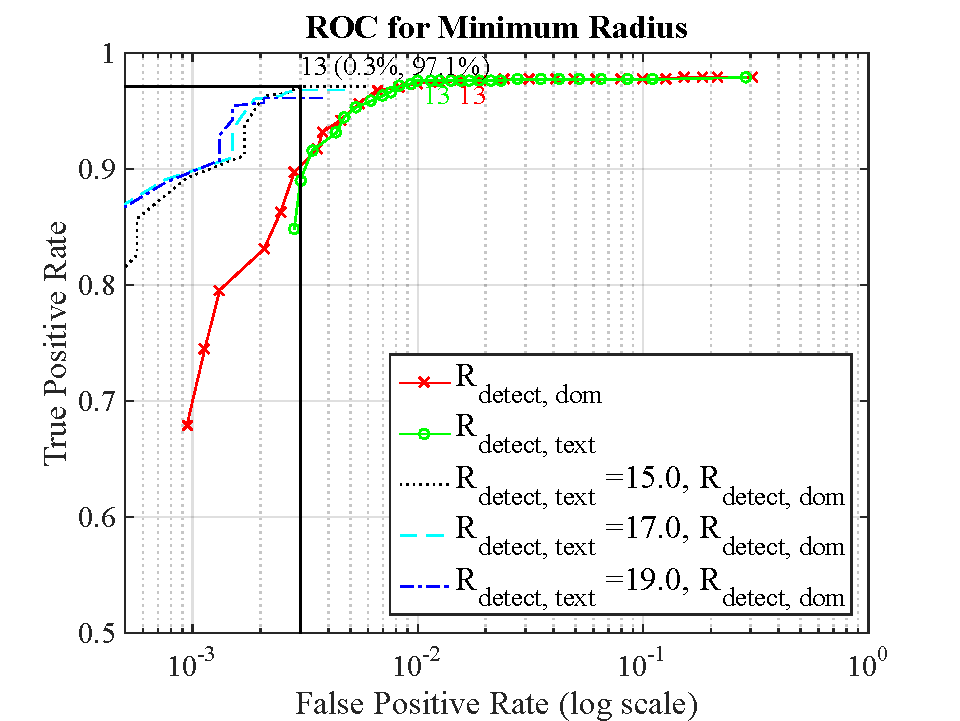
\includegraphics[width=.5\textwidth]{fig/roc}
  \caption{ROC for DOM, TEXT, DOM \& TEXT}
  \label{fig:roc}
\end{figure}

With the learned model, in Section ~\autoref{s:measurement} 
detect on the four dataset that we obtained and
manually label the results. In our detection, we want a low false positive rate,
therefore, we use the FPR = 0.1\%, TRP = 92\% in ~\autoref{fig:roc}. This yields
to $R_{detect, dom} = 16$, $R_{detect, text} = 20$.


\subsection{Efficiency Comparison}
\label{ss:efficiency}
While we can achieve similar false positve rate and true positive rate compared
to past approaches, we argue that, our approach is much more efficient than past
approaches and is light-weight enough to be deployed on user browser.
\XXX{Table} is a comparison of time complexity and number of rounds that the
documents need to be processed (each time they get smaller amount of document,
though). Let $N$ denote the number of total urls collected, $M$ denoete the
number of cloaking websites. The time complexity is \XXX{Plot}.



For simhash computation, we implements a browser extension which exposes
negligible overhead to user. We 

\XXX{the table comparing our approach with past cloaking detection approaches}
\XXX{the ability of simhash in measuring difference}.




